\documentclass[fontsize = 11pt,a4paper]{article}
\usepackage{fancybox,fancyhdr} 
\usepackage[utf8]{inputenc}
\usepackage[russian]{babel}
\usepackage{multicol}
\usepackage{titlesec}
\usepackage{amsmath}
\usepackage{indentfirst}
\usepackage{graphicx}
\usepackage{subcaption}
\usepackage{wrapfig}



\setlength\parindent{12pt}
\usepackage[left=2cm,right=2cm,
    top=2cm,bottom=2cm]{geometry}
\title{\textbf{A Celestial-Mechanical Model for the Tidal Evolution\\
of the Earth-Moon System Treated as a Double Planet}}
\author{\textbf{A. A. Zlenko*}}
\date{\emph{Moscow Automobile and Roadway State Technical University, Moscow, Russia}\\
Received May 6, 2014; in final form, May 21, 2014}
\begin{document}
\maketitle

\thispagestyle{fancy}
\fancyhead[L]{\tiny \emph{ISSN 1063-7729, Astronomy Reports, 2015, Vol. 59, No. 1, pp. 72–87. \copyright Pleiades Publishing, Ltd., 2015.\\
Original Russian Text \copyright A.A. Zlenko, 2015, published in Astronomicheskii Zhurnal, 2015, Vol. 92, No. 1, pp. 80–96.\newline \newline}}


\fancyfoot[L] {*E-mail: zalaf121@mail.ru}
\renewcommand{\footrulewidth}{0.4pt}


\makeatletter
\def\headrule{{\if@fancyplain\let\headrulewidth\plainheadrulewidth\fi
\hrule\@height\headrulewidth\@width\headwidth
\vskip 2pt% 2pt between lines
\hrule\@height.5pt\@width\headwidth% lower line with .5pt line width
\vskip-\headrulewidth
\vskip-1.5pt}}
\makeatother


\indent\vbox{
\noindent\textbf{Abstract}—A celestial-mechanical model for the motion of two viscoelastic spheres in the gravitational
field of a massive point is considered, treating them as a double planet. The spheres move along quasicircular
orbits in a single plane, with their rotational axes perpendicular to this plane. The deformation of
the spheres is described using the classical theory of small deformations. A Kelvin–Voigt model is adopted
for the viscous forces. A system of evoutionary equations is obtained and 
lied to analyze the joint
translational–rotational tidal evolution of the Earth and Moon in the gravitational field of the Sun. This
system has been numerically integrated several billion years into the past and into the future. The results
are compared with the predictions of other theories, paleontological data, and astronomical observations.
\\
\\
\textbf{DOI}:10.1134/S1063772915010096
}
\begin{multicols}{2}

 \centerline{ 1. INTRODUCTION}
~\\
\indent The theory of tides originated with work by Newton
and Laplace. The main achievements in this
area were collected, systematized, and analyzed by
Darwin [1], and further developed by MacDonald [2],
who studied the evolution of the Earth–Moon system
without including the influence of the Sun. Goldreich
[3] used the method of MacDonald to investigate the
oblateness of the Earth and the influence of solar
tides, but neglecting the ellipticity of the lunar orbit,
and correctly averaged the equations of motion using
three time scales.\\
\indent The method of MacDonald was then used in various
other studies. Beletskii [4] investigated the tidal
evolution of the inclinations and rotations of celestial
bodies. Webb [5] studied the evolution of the
Earth–Moon system based on the ocean tides and
compared his results with the model of Goldreich [3].
Krasinsky [6] combined the methods of MacDonald
and Goldreich to reconstruct a dynamical history of
the Earth–Moon system. Touma andWisdom [7] developed
various models for tidal phenomena in detail.
It was shown that the evolution of the Earth–Moon
system based on the models of Darwin–Mignard and
Darwin–Cowley–Goldreich is essentially equivalent
to that predicted by the model of Goldreich.\\
\indent Efroimsky and Lainey [8] considered the effective
dissipation function Q, which is proportional to the
tidal frequency to the power $\alpha$. They studied the tidal
evolution of the Martian moon Phobos for $\alpha$ = 0.2, 0.3, 0.4. Note that $\alpha = 0$ in the model of MacDonald
and $\alpha$ = -1 in the model of Mignard [9, 10]. The
main distinguishing property of the approach proposed
by Ferraz-Mello et al. [11] is that, in contrast to
many studies based on the theory of Darwin, different
coefficients are introduced for the harmonics of the
tidal wave, instead of one Love number. A critical
analysis of the mathematical formulas in the above
theories describing the tidal moments, slowing of
planetary rotation, and the delay angle, as well as the
accuracy and range of applicability of the theories and
connections with rheological models, are considered
by Efroimsky and Williams [12] and Efroimsky and
Makarov [13]. Note that the qualitative conclusions
derived for the simpler MacDonald theory essentially
remain correct [12].\\
\indent The subsequent development of tidal theories is
concerned with the creation of rheological models.
Churkin [14–16] established a generalized theory of
the Love number and applied it to the rheological
models of Guk, Maxwell, Voigt, and others. His
theory for the rotation of the inelastic Earth was applied
to a Voigt model for the Earth’s interior, and
numerical estimates of rheological corrections to the
precession, nutation, and axial rotation of the Earth
were obtained. Efroimsky [17] introduced complex
Love numbers as a function of the tidal frequency to
study tides in the case of a rotational–orbital resonance
between a planet and one of its satellites.
Vil’ke [18] developed a method for separating motions
and averaging in systems with an infinite number
of degrees of freedom, aimed at studying the
motions of deformable bodies using a classical linear
\end{multicols}

\pagebreak

\begin{multicols}{2}
elasticity theory for small deformations and a Kelvin–
Voigt model for the viscous forces. This method
was used to investigate the evolution of the orbital
and rotational motions of a viscoelastic planet in a
central Newtonian force field [19, 20]. The model for a
celestial body of Markov and Minyaev [21] includes
an isotropic, viscoelastic layer and a rigid core. A
qualitative analysis of the motion of the moons of
Mars is given, and the model parameters were refined
based on the observations of the secular acceleration
of Phobos. Vil’ke and Shatina [22] studied the tidal
evolution of the motion of the Earth–Moon system in
the gravitational field of the Sun, treating the Moon
as a point mass.
Let us now turn to our model describing a double
planet [23–25].
\begin{center}
 2. MATHEMATICAL MODEL\\
FOR THE MOTION OF TWO VISCOELASTIC\\
SPHERES IN THE GRAVITATIONAL FIELD\\
OF A FIXED CENTRAL BODY
\end{center}
 \centerline{\emph{2.1. Formulation of the Problem}}
In the unperturbed motion, the barycenter C of the
two uniform rigid spheres $O_{1}$  and $O_{2}$ with masses m1
and m2 moves in a circular, Keplerian orbit in a fixed
plane in the gravitational field of a stationary massive
point mass M. The spheres $O_{1}$ and $O_{2}$, in turn,
move in circular Keplerian orbits about the barycenter
C in the plane of its motion. The spheres rotate
with specified constant angular speeds about axes
passing through their centers of mass perpendicular
to the plane of their orbital motion. All four motions
are independent of each other. This formulation of
the problem is possible because we have made the
assumptions

$m2 \ll m1 \ll M; r_{i0} \ll  R_{2} \ll R_{1}, $ \hfill(1)\\
where $r_{i0}$ (i = 1, 2) are the radii of the spheres, $R_{1}$
is the distance from the gravitating center to the
barycenter, and $R_{2}$ is the distance between the centers
of mass of $O_{1}$ and $O_{2}$ (we will further identify
the names of the spheres with their centers of mass).
These assumptions are satisfied, for example, by the
Sun–Earth–Moon system.\\
In the perturbed motion, we treat the spheres as
uniform, isotropic, viscoelastic bodies. Perturbations
arise due to the deformation of the bodies in response
to the centrifugal and gravitational forces. Since we
are studying evolutionary motions, we assume that
the centers of mass of the spheres move along quasicircular
orbits.\\
To describe the motion, we specify an inertial
coordinate frame OXY Z fixed to the gravitating
center O, with the spheres moving in the OXY
plane. We specify Koenig coordinate systems ${O_i}{X_i}{Y_i}$
with the points ${O_i}$ (i = 1, 2). The position of the barycenter C in the OXY Z system is specified by
the vector ${R_1} = \vec{OC} ({R_1} \cos {\lambda_1}, {R_1} \sin {\lambda_1}$, 0), where
$|{R_1}| = {R_1}$, and ${\lambda_1}$ is the angle between ${R_1}$ and the
OX axis. The position of ${O_2}$ relative to ${O_1}$ in the
${O_1}{X_1}{Y_1}{Z_1}$ frame is specified by the vector ${R_2} = {O_1}{O_2}({R_2} \cos {\lambda_2}, {R_2} \sin {\lambda_2}, 0)$, where 
$|{R_2}| = {R_2}$,  and
${\lambda_2}$ is the angle between ${R_2}$ and the $O{X_1}$ axis. The
deformed state of the bodies is described by the classical
theory of elasticity for small deformations. We
adopted a Kelvin–Voigt model for the viscous forces,
with the dissipation function ${D_i}[{\dot{u}_i}]$ proportional to
the elastic-force function ${W_i}[{\dot{u}_i}]$, with the coefficient
of proportionality ${X_i}$ (the viscosity coefficient):
${D_i}[{\dot{u}_i}] = {X_i}{W_i}[{\dot{u}_i}$], (2)
where ${u_i}({r_i}, t)$ is the shift in the points of the body ${O_i}$
due to the deformations, ${\dot{u}_i} = d{u_i}/dt$ (here and below,
a dot above a quantity denotes a time derivative), and
${r_i}$ is the radius vector of the points in a sphere relative
to the center ${O_i}$ in the undeformed state.
\\
\indent The rotating spheres are associated with their own
coordinate systems ${O_i}{X_{ii}}{Y_{ii}}{Z_{ii}}$, where the ${O_i}{Z_{ii}}$ axis
is perpendicular to the orbital plane (the ${O_i}{Z_i}$ and
${O_i}{Z_{ii}}$ axes coincide). The positions of the points in
the viscoelastic sphere ${O_i}$ in the OXY Z coordinate
system are determined by the vector field
${\zeta_i}({r_i},t) = \vec{O{O_i}} + {\Gamma_i}({\varphi_i})({r_i}+{u_i}({r_i},t))$,
where
$ {\Gamma_i}({\varphi_i}(t)) =
 \begin{pmatrix} 
\cos{\varphi_i} & -\sin{\varphi_i}  & 0\\
\sin{\varphi_i} & \cos {\varphi_i} & 0\\
0 & 0 & 1
\end{pmatrix}
.(4)$
Here,${\Gamma_i}$ is the orthogonal operator for the translation
from the Koenig coordinates ${O_i}{X_i}{Y_i}{Z_i}$ to the
coordinates ${O_i}{X_{ii}}{Y_{ii}}{Z_{ii}}$ and ${\varphi_i}$ is the rotation of the
${O_i}{X_{ii}}{Y_{ii}}{Z_{ii}}$ system about the ${O_i}{Z_{ii}}$ axis (${\varphi_i}$ is the
angle between the ${O_i}{X_i}$ and ${O_i}{X_{ii}}$ axes).
In order to uniquely determine the positions of the
centers of mass of the spheres ${O_i}$ in the ${O_i}{X_{ii}}{Y_{ii}}{Z_{ii}}$
coordinate systems as the spheres move by ${\zeta_i}({r_i}, t)$,
we imposed the following conditions (relations) on
this motion:\\
\indent
$\int\limits_{V_i} {u_i}d{v_i} = 0,$
$\int\limits_{V_i} curl{u_i}d{v_i} = 0$

$(d{v_i} = d{x_{ii}}d{y_{ii}}d{z_{ii}})$,
\\ where ${V_i} = \{|{r_i}| < {r_{i0}} \}$ is the region occupied by Oi
in the undeformed state.
\end{multicols}

\pagebreak
\begin{multicols}{2}
The functional for the kinetic energy of the system
has the form
$T = \frac{1}{2}m{\dot{R}^2_1} + \frac{m1m2}{2m}{\dot{R}^2_2} + \frac{1}{2}\sum_{i=1}^{2}{J_i}[{u_i}]{\dot{\varphi}_i}^2 + 2{G_i}{\dot{\varphi}_i}+{T_{0i}})$,
\\ where 
${J_i}[{u_i}] $= $\int\limits_{V_i} [{e_3}\times ({r_i} + {u_i})]^2 {\rho_i}d{v_i}$,
${G_i} = \int\limits_{V_i}[{e_3} \times ({r_i} + {u_i}),\dot{{u_i}}]{\rho_i}d{v_i}, $
${T_{0i}} = \int\limits_{V_i} (\dot{{u_i}}^2) {\rho_i} d {v_i},$
${e_3}$ is the unit vector for the $O_i Z_{ii}$ axis perpendicular
to the OXY plane, and ${\rho_i}$ is the density of the sphere
$O_i$.\\
The potential energy associated with the gravitational interactions is given by\\
$\Pi=\Pi_1 + \Pi_2 + \Pi_3$, \\
where $\Pi_1 = -f \int\limits_{V_i} \{(R_1 - m_2/m)R_2$ \\
$+\Gamma_1 (r_1 + u_1)]^2\}^{-1/2}\rho_1 d v_1$\\
is the energy associated with the interaction between
the gravitating center and the viscoelatic body $O_1$,
$\Pi_2 = -f \int\limits_{V_2} \{(R_1 + m_1/m)R_2$ \\
$+\Gamma_2 (r_2 + u_2)]^2\}^{-1/2}\rho_2 d v_2$\\
is the energy associated with the interaction between
the gravitating center and the viscoelatic body $O_2$,
$\Pi_3 = -f  \int\limits_{V_i}\int\limits_{V_2} \{(R_2 +\Gamma_2(r_2 + u_2)$ \\
$-\Gamma_1 (r_1 + u_1)]^2\}^{1/2}\rho_1\rho_2 d v_1d v_2$\\
is the energy associated with the deformable spheres
$O_1$ and $O_2$, f = GM, G is the gravitational constant,
and $m = m_1 + m_2$. Taking into account the condition
(1) and neglecting terms of order $(R_2/R_1)^3(m_2/m)^3$
and higher order in smallness in the potential energy,
and leaving only terms that are linear $u_i$, we obtain
$\Pi = fm/R_1 - G{m_1}{m_2}/R_2 + {\Pi _\rho}$ (8)\\
$\Pi_\rho = \sum\limits_{k=1}^{2} \sum\limits_{i=1}^{2} f_{ki}/ {R_k}^3\int\limits_{V_i}[{r_i}{u_i}$ (9) \\
$-3(\xi_{ki},r_i)(\xi_{ki},u_i)]\rho_idv_i$,\\
$f_{1i} = f$,   $f_{2i} = Gm_{3-i}$, \\
$\xi_{ki} = \tau_{ki}[\cos(\lambda_k - \phi_i),\sin(\lambda_k - \phi_i),0],$\\
$\tau_{21} = -1,$   $\tau_{ki} = 1$   $(k \neq 2, i \neq 1).$ \\
Following [22], we introduced canonical Poincar$\dot{e}$
variables $\lambda_k, \Lambda_k$ (k = 1, 2 to describe the motion of
the barycenter and centers of mass $O_i$:
$\Lambda_1 = m (fR_1)^{1/2}$,   $\Lambda_2 = m_r (f_0R_2)^{1/2}$ , (10)\\
where $m_r = m_1m_2/m, f_0 = Gm.$\\
To describe the rotational motion of the bodies, we\\
used the Andoyer canonical variables $\varphi_i, I_i $  (i = 1, 2):\\
$I_i = J_i[u_i]\dot{\varphi_i} + G_i$,    (11)\\
where $J_i[u_i]$ and $G_i$ is defined in (6). \\
The equation of motion was written in the form of
the Routh equations \\
$\dot{\Lambda_k} = -  \frac{\partial\Re }{\partial{\lambda_k}},$
$\dot{\lambda_k} = \frac{\partial\Re }{\partial{\Lambda_k}},$
$\dot{I_i} = -  \frac{\partial\Re }{\partial{\varphi_i}},$ (12) \\

$\dot{\varphi_i} = -  \frac{\partial\Re }{\partial{I_i}},$
$\frac{d}{dt} {\nabla_{\dot{u_i}}}\Re - {\nabla_{u_i}}\Re - {\nabla_{\dot{u_i}}}D_i = 0.$
Here, $\Re$ is the Routh function, which has the form\\
$\Re = - \frac{{f^2}{m^3}}{2{\Lambda_1}^2} - \frac{{f_0}^2{m_r}^3}{2{\Lambda_2}^2}$ \hfill (13)\\
$+  \sum\limits_{i=1}^{2} \{ \frac{{I_i}^2}{2A_i} -\frac{{I_i}^2}{2{A_i}^2}J_{i1}[u_i] $\\
$- \frac{I_i}{A_i}( e_3, \int\limits_{V_i} (r \times \dot{u_i}) dv) + W_i[u_i]\} + {\Pi_\rho}$\\
where $A_i$ = 0.4${m_i}{r^2_{i0}}$ is the moment of inertia of the
undeformed sphere $O_i$,\\
$J_{i1}[u_i] = 2  \int\limits_{V_i}[(r_i, u_i) - (e_3, r_i)(e_3, u_i)]\rho_idv_i,$(14)\\ 
and an expression for $\Pi_\rho$ is give by (9). \\
\indent The equations of motion admit the integral of the
angularmomentum. When the Routh function (13) is
written out in detail, it can be shown that the angular
variables $\lambda_k$ and $\varphi_i$ appear in this function in the
combination $\psi_{ki} = \lambda_k - \varphi_i$. It follows that \\
$\dot{I}_i = - \frac{\partial\Re}{\partial\varphi_i} = - \sum\limits_{k=1}^{2}\frac{\partial\Re}{\partial\psi_{ki}}\cdot
\frac{\partial\psi_{ki}}{\partial{\varphi_i}} = \sum\limits_{k=1}^{2} \frac{\partial\Re}{\partial\psi_{ki}}$, \hfill (15)\\
$\dot{\Lambda_k} = -  \frac{\partial\Re }{\partial{\lambda_k}} = - \sum\limits_{i=1}^{2} \frac{\partial\Re}{\partial\psi_{ki}} 
\cdot \frac{\partial\psi_{ki}}{\partial{\Lambda_k}} = - \sum\limits_{i=1}^{2}\frac{\partial\Re}{\partial\psi_{ki}},$\\
$\dot{I_1} + \dot{I_2} + \dot{\Lambda_1} + \dot{\Lambda_2}$\\
$ = \sum\limits_{i=1}^{2} \sum\limits_{k=1}^{2} \frac{\partial\Re}{\partial\psi_{ki}} -  \sum\limits_{k=1}^{2} \sum\limits_{i=1}^{2}
 \frac{\partial\Re}{\partial\psi_{ki}} = 0,$ \\
${I_1} + {I_2} + {\Lambda_1} + t{\Lambda_2} = K_0 = const.$\\
 \centerline{\emph{2.2.Finding the Displacements of Points\\
in the Bodies due to their Deformation}}
\indent The system (12) cannot be integrated in explicit
form, since this is a quite complex system of differential
equations. Therefore, we applied the method
for separating motions in systems with an infinite
number of degrees of freedom [18]. Since we assumed
the rigidity of the elastic spheres $O_i$ were high, we
introduced the small parameters $\varepsilon_i$, proportional to
the ratio of the squares of the angular velocity of
rotation of a sphere at the initial time and of the lowest
frequency for the intrinsic elastic vibrations of the
sphere. The displacements $u_i$ are small, and can be
represented as a series in powers of $\varepsilon_i$:\\
$u_i(r_i,t) = \varepsilon_i u_{i1}(r_i,t) +  \varepsilon_i^2 u_{i2}(r_i,t) + ...,$\hfill (16) \\
$\varepsilon_i = \rho_i r^2_{i0} \varphi^2_i(0) / E_i,$ \hfill (17) \\
where $E_i$ is the Young’s modulus for the body $O_i$.\\
If $\varepsilon_i  = 0$, then $u_i(r_i, t) = 0$, and the equations of
the unperturbed motion follow from (12):\\
$\dot{\Lambda_1} = \dot{\Lambda_2} = \dot{I_1} = \dot{I_2} = 0,$\\
$\dot{\lambda_1} = \omega_1$,   $\dot{\lambda_2} = \omega_2$  $\dot{\varphi_1} = \omega_3$  $\dot{\varphi_2} = \omega_4$\\
where \\
$\omega_1 = \frac{f^2m^3}{\Lambda^3_1}$,    $\omega_2 = \frac{f^2_0 m^3_r}{\Lambda^3_2}$ \hfill (19)\\
$\omega_3 = \frac{I_1}{A_1}$,  $\omega_4 = \frac{I_2}{A_2}$.\\
In this case, the center of mass of the two bodies C
moves along a circular orbit about the fixed center
O with a constant angular velocity $\omega_1$, the bodies
$O_i$ move along circular orbits about their center of
mass C with a constant angular velocity $\omega_2$, and the
bodies $O_1$ and $O_2$ rotate on their axes with constant
angular velocities $\omega_3$ and $\omega_4$, normal to their orbital
plane passing through their centers of mass. \\
\indent It can be shown that, after the intrinsic vibrations
of the viscoelastic spheres have died away, including
only the first term $\varepsilon_i u_{i1}$ in the expansion of $u_i(r_i, t)$ in
powers of $\varepsilon_i$ in (16), the last equations in (12) reduce
to the two relations\\
$\nabla_{u_i}W_i[\varepsilon_i u_{i1} + \chi_i \varepsilon_i \dot{u_{i1}}]$
$ = \rho_i \{ \omega^2_{2+i} [ r_i - (e_3,r_i)e_3]$\\
$+  \sum\limits_{k=1}^{2} (f_{ki} / R^3_k)[3(\xi_{ki},r_i) \xi_{ki} - r_i] \}$ (i = 1, 2),\\
where\\
$\nabla_{u}W_i[\varepsilon_i u] = \frac{\rho_ir^2_{i0}\dot{\varphi^2_i}(0)}{2(1 + v_i)}$\hfill (21)\\
$ \times (\frac{1}{1 - 2v_i}\nabla div u + \Delta u),$ \\
and $v_i$ is the Poisson coefficient for the matter in the
sphere $O_i$.\\
Equation (20) can be written in the form\\
${\varepsilon_i} \nabla_{u_i} W_i [u_{i1} + \chi_i \dot u_{i1}]$ \hfill (22) \\
$=\rho_i [\omega^2_{2+i}(2r_i/3 + B_o r_i) +  \sum\limits_{k=1}^{2} 3 (f_{ki}/R^3_k)B_{ki} r_{i}],$\\
where\\
$B_0 = 
\begin{pmatrix} 
1/3 & 0 &  0 \\
0 & 1/3 & 0 \\
0 & 0 & -2/3
\end{pmatrix}, $
\\
$B_{ki} = \frac{1}{6}
\begin{pmatrix} 
3cos 2 \psi_{ki} + 1  & 3 sin 2 \psi_{ki} &  0 \\
3 sin 2 \psi_{ki} & -3cos 2 \psi_{ki} + 1 & 0 \\
0 & 0 & -2
\end{pmatrix}.$\\
All the quantities in the right-hand side of (22) are
calculated for the unperturbed motion.\\
Taking into account the fact that the stresses on
the surfaces of the deformable bodies $O_i$ are zero (i.e.,
the boundary conditions for the functions $u_{i1}(r_i, t)$
have the form $\sigma_{in} = 0$), with accuracy to within firstorder
terms in the small quantity $\chi_i$, the solution of
(22) has the form\\
$u_i(r_i,t) \approx \varepsilon_i u_{i1} = u_{i11} + u_{i12} + u_{i13},$ \hfill (23) \\
$u_{i11} = \rho_i / E_i \omega^2_{2 + i} [-2/3(d_{i1} r^2_i + d_{i2} r^2_{i0})$\\
$+ a_{i1}(B_0 r_i, r_i) + (a_{i1} r^2_i + a_{i2} r^2_{i0})B_0]r_i,$\\
$u_{i12} = 3 \rho_i / E_i \sum\limits_{k=1}^{2} f_{ki} R^{-3}_k [a_{i1}(B_{ki}r_i,r_i)r_i$\\
$ + (a_{i2}r^2_i + a_{i3} r^2_{i0}) B_{ki}r_i],$\\
$u_{i13} = -3 \rho_i / E_i \sum\limits_{k=1}^{2} f_{ki} R^{-3}_k \chi_i (\omega_k - \omega_{2+i})$\\
$\times [a_{i1}(\frac{\partial B_{ki}}{\partial \psi_{ki}} r_i, r_i)r_i + (a_{i2}r^2_i +  a_{i3} r^2_{i0}) \frac{\partial B_{ki}}{\partial \psi_{ki}} r_i ], $\\
where\\
$d_{i1} = \frac{(1 + v_i)(1 - 2v_i)}{10(1 - v_i)},$\\
$d_{i2} =- \frac{(3 - v_i)(1 - 2v_i)}{10(1 - v_i)},$\\
$a_{i1} =- \frac{1+ v_i}{5 v_i + 7},$   $a_{i2} =- \frac{(1+ v_i)(2 + v_i)}{5 v_i + 7}. $\\
The structure of $u_i(r_i, t)$ is such that the first term
$u_{i11}$ describes axially symmetrical, elastic deformation
of the sphere $O_i$, which is compressed by the
action of the centrifugal force associated with the
rotation about the $O_iZ_{ii}$ axis passing through the
center of mass. The second term $u_{i12}$ characterizes
the deformation of the body $O_i$ due to the external
gravitational fields of the two other bodies. These
fields also give rise to gravitational tides, given by the
third term $u_{i13}$, which contains the viscosity coefficient
$\chi_i$ and influences the evolution of the motion.

\centerline{\emph{2.3. Simplification and Averaging\\
of the Equations of Motion}}
Let us write the canonical equations (12) in more
detail, taking into account the Routh function and the
displacements $u_i(r_i, t) \approx \varepsilon u_{i1}:$\\
$\dot\Lambda_k = 3  \sum\limits_{i=1}^{2} \rho_i f_{ki} R^{-3}_k$ \hfill (24) \\
$ \times \int\limits_{V_i}[(\frac{\partial{\xi_{ki}}}{\partial{\lambda_k}},ri)(\xi_{ki} \varepsilon_i u_{i1})$\\
$+ (\xi_{ki}, r_i) (\frac{\partial{\xi_{ki}}}{\partial{\lambda_k}}, \varepsilon_i u_{i1})] dv_i,$\\
$\dot\lambda_k  = \omega_k - 3 \sum\limits_{i=1}^{2} \rho_i f_{ki} R^{-4}_k \partial R_k / \partial \Lambda _k$ \hfill (25)\\
$ \times  \int\limits_{V_i} [ r_i \varepsilon_i u_{i1}) - 3(\xi_{ki}, r_i)(\xi_{ki},\varepsilon_i u_{i1})] d v_i,$ \\
$\dot I_i = 3 \rho_i \sum\limits_{k=1}^{2}  f_{ki} R^{-3}_k $ \hfill (26) \\
$ \times  \int\limits_{V_i} [(\frac{\partial{\xi_{ki}}}{\partial{\varphi_i}}, r_i)(\xi_{ki}, \varepsilon_i u_{i1})$ \\
$ + ( \xi_{ki}, r_i) (\frac{\partial{\xi_{ki}}}{\partial{\varphi_i}},  \varepsilon_i u_{i1})]  d v_i,$ \\
$\dot \varphi_i = \omega_{2 + i} - 2 {\rho_i} \frac{\omega_{2 + i}}{A_i}$ \hfill (27) \\
$\times \int\limits_{V_i}[ (r_i,  \varepsilon_i u_{i1}) - (e_3,r_i)(e_3, \varepsilon_i u_{i1})] d v_i$ \\
$- \frac{\rho_i}{A_i}[e_3,\int\limits_{V_i}(r \times \varepsilon_i  \dot u_{i1})d v_i].$\\
Subsituting the resulting variables (23) into the
equations of motion (24)–(27) and calculating the
necessary cumbersome integrals yields the system of
equations of motion\\
$\dot\Lambda_k  = -18 \sum\limits_{i=1}^{2} \rho ^2_i / E_i D_{i2} m_{3-i} \omega^2_k / m$ \hfill (28) \\
$\times \{ \chi_i {(m_{3-i}/m)}^{2k-3} \omega^2_k(\omega_k - \omega_{2+i})$\\
$+ \omega^2_{3-k}[(-1)^{2-k}0.5 \sin \tau + \chi_i ( \omega_{3-k} -  \omega_{2+i}) \cos \tau] \},$\\
$\dot I_i = 18 \rho^2_i / E_i D_{i2} \chi_i[ {\omega^4}_1(\omega_1 - \omega_{2 + i})$ \hfill (29) \\
$+ {(m_{3-i} / m) }^2 {\omega^4}_2(\omega_2 - \omega_{2 + i})$\\
$+ m_{3 - i} / m \omega^2_1 \omega^2_2 (\omega_1 + \omega_2 - 2 \omega_{2+i} \cos \tau],$ \\
$\dot\Lambda_k = \omega_k + 6 \sum\limits_{i=1}^{2} \rho ^2_i / E_i D_{i2}{( m_{3-i} / m)} ^ {k-1}$ \hfill (30)\\
$\times \Lambda_k ^ {-1} \omega_k ^2 \{ \omega_{2+i}^2 + 6 {( m_{3-i} / m)}^{k-1} \omega_{k}^2$\\
$+ 3 {(m_{3-i}/ m)} ^{2-k} \omega_{3-k}^2[0.5 + 1.5 \cos \tau$\\
$+ 3 {(-1)}^{k-1} \chi_i ( \omega_{3-k} - \omega_{2 + i}) \sin \tau ] \},$\\
$\dot \varphi_i = \omega_{2 + i} - 2 \rho_i ^2 / E_i {A_i} ^{-1} \omega_{2 + i} [ D_{i2}(\omega^2_1$ \hfill (31) \\
$+ m_{3-i}/m\omega^2_2) + 2/3(2 D_{i1} + D_{i2}) \omega ^2 _{2 + i}],$\\
where\\
$D_{i1} = \frac{8\pi r^7_{i0}(1-2v_i)(4-3v_i)}{525(1-v_i)},$\\
$D_{i2} = \frac{4\pi r^7_{i0}(1+v_i)(9v_i+13)}{105(5v_i+7)},$\\
$\tau = 2 (\lambda_2 - \lambda_1).$
The right-hand sides of these equations do not
depend on $\varphi_i$. Since the equations (31) depend only
on $\lambda_k$ and $I_i$, they can be separated from the remaining
equations and integrated after the integration of\\
(28)-(30). If $\omega_1$ = $\omega_2$, the angular variable $\tau$ is a rapid
variable, and averaging Eqs. (28)-(30) over$\tau$ yields
the evolutionary system of equations \\
$\dot\Lambda_k  = -18 \omega_k^4 \sum\limits_{i=1}^{2} \chi_i \rho_i^2 / E_i$ \hfill (32) \\
$\times D_{i2}{(m_{3-i}/m)}^{2k-2} (\omega_k - \omega_{2+i}),$\\
$\dot{I_i} = 18 \chi_i \rho_i^2 / E_i D_{i2}[\omega^4_1(\omega_1 - \omega_{2+i}) $\hfill (33) \\
$+ {(m_{3-i}/m)}^{2} \omega^4_2 (\omega_2 - \omega_{2+i})],$\\
$\dot\lambda_k = \omega_k + 6 \Lambda_k^{-1} \omega_k ^2$ \hfill (34) \\
$\times \sum\limits_{i=1}^{2} \rho_i^2 /  E_i D_{i2} {( \frac{m_{3-i}}{m})}^{k-1}$\\
$\times [ \omega^2_{2+i} + {(m_{3-i} / m)}^{k-1} \omega^2_k$\\
$+1.5 {(m_{3-i} / m)}^{2-k}\omega^2_{3-k}].$\\
The right-hand sides of the averaged equations do
not depend on $\lambda_k$, and Eq. (34) can be separated
from (32)-(33) and integrated after the solution of the
independent system (32)-(33).\\
Since\\
$\Lambda_1 = {(f^2m^3\omega^{-1}_1)}^{1/3},$\\
$\Lambda_2 = {(G^2{m_1}^3 {m_2}^3 m^{-1} \omega^{-1}_2)}^{1/3},$\\
$\omega_3 = I_1 / A_1, \omega_4 = I_2/A_2,$\\
the system (32)-(33) can be written in the more
“intuitive” variables $\omega_j$ (j = 1-4):\\
$\dot \omega_1 = c_1 \omega^{16/3}_1 [k_1(\omega_1 - \omega_3) + k_2 ( \omega_1 - \omega_4)],$ \hfill (35)\\
$\dot \omega_2 = c_2 \omega^{16/3}_2 [k_1{(m_2 / m)}^2 (\omega_2 - \omega_3)$\\
$ + k_2 {(m_1 / m)}^2 ( \omega_2 - \omega_4)],$\\
$\dot \omega_3 = c_3 k_1 [ \omega^{4}_1 (\omega_1 - \omega_3) +  {(m_2 / m)}^2 (\omega_2^4) (\omega_2 - \omega_3)],$\\
$\dot \omega_4 = c_4 k_2 [ \omega^{4}_1 (\omega_1 - \omega_4) +  {(m_1 / m)}^2 (\omega_2^4) (\omega_2 - \omega_4)],$\\
where
$k_i = \chi_i \rho_i^2 / E_i D_{i2}, c_1=54f^{-2/3}m^{-1},$\hfill (36)\\
$c_2 = 54G^{-2/3} m^{1/3} m^{-1}_1 m^{-1}_2,$ \\
$c_3 = 18A^{-1}_1, c_4 = 18A^{-1}_2$\\
The system (35) has the first integral\\
$3c^{-1}_1 {\omega_1}^{-1/3} + 3c^{-1}_2 {\omega_2}^{-1/3}$ \hfill (37) \\
$+ {c_3}^{-1} \omega_3 +  {c_4}^{-1} \omega_4 = K_0.$\\
Thus, we obtained the independent system of firstorder
ordinary differential equations (35) to investigate
the evolution of the slow variables: the angular
velocity of the orbital motion of the center of mass
of the binary planet (two viscoelastic bodies) about
the gravitating center $\omega_1$, the angular velocity of the
planets about their common center of mass  $\omega_2$, and
the angular rotational velocities of the two bodies
$\omega_3$ and $\omega_4$. The right-hand sides of these equations
all contain the viscosity coefficient $\chi_i$ through the
coefficients ki. If $\chi_i$ is zero, there is no tidal evolution
of the system.
\begin{center}
 3. NUMERICAL INTEGRATION\\
OF THE EQUATIONS OF MOTION
\end{center}
 \centerline{\emph{3.1. Input Data}}
The system (35) was numerically integrated using
theMATLAB R2013a programme package. We took
the Sun to be the fixed gravitating center, the first
body to be the Earth, and the second body to be the
Moon. We took the following data from [26] for the
current epoch:\\
\indent -G = 6.67428 $ \times {10}^{11} {m}^3 {kg}^{-1} {s}^{-2}$ is the gravitational
constant,\\
\indent -f = $GM_S = 1.32712442099 \times 10^{20} m^3/ s ^2$ is
the heliocentric gravitatonal constant,\\
\indent -$GM_E = 3.986004418 \times 10^{14} m^3 / s^2$ is the geocentric
gravitational constant,\\
\indent $-M_M / M_E = 1.23000371 \times 10^{-2}$ is the ratio of
the masses of theMoon $M_M$ and the Earth $M_E.$\\
We also took the following quantities at the current
epoch from [27]:\\
\indent-the duration of a single orbit of the \hfill (38)\\
Earth-Moon system around the Sun, equal 
to a sidereal year, $T_1$ = 365.25636296 d,\\
\indent-the duration $T_2$ of a single orbit of theMoon
about the Earth, equal to a sidereal month and
also equal to the rotational period of the Moon
$T_4$; i.e., $T_2 = T_4$ = 27.3216616 d,\\
\indent-the duration of an Earth day $T_3$= 86 400 s,\\
\indent-the radius of the Moon $r_20$ = 1737.4 km\\
\indent-the radius of the Earth $r_10$ = 6371.032 km.
We used the units of measurement
\indent-for mass the solar mass M = $M_S$ = 1, \hfill (39) \\
\indent-for length L = ${10}^8$ m,\\
\indent-for time T = 31 558 149.759744 s, equal to
one year.\\
In these new units\\
G = f = 1.321705528131173 $\times {10}^{11}$, \hfill (40)\\
$m_1$ = $M_E$ = 3.003489616313853 $ \times 10^{-6}$,\\
$m_2$ =$ M_M$ = 3.694303371012516$ \times 10^{-8}$,\\
m = 3.040432650023978  $\times  10^{6}$,\\
$A_1$ = 4.876471597254109  $\times  10^{9}$,\\
$A_2$ = 4.460588721066945 $\times 10^{12}$,\\
where $A_i$ are the moments of inertia (13).\\
We find from (36) the values\\
$c_1$ = 6.844923013835195 $\times {10}^{-1}$, \hfill (41) \\
$c_2$ = 2.717213270640726 $\times {10}^{5}$,\\
$c_3$ = 3.691193446125189 $\times {10}^{9}$,\\
$c_4$ = 4.035341773382441 $\times {10}^{12}$.\\
The initial values for $\omega_i$ were taken to be $\omega_i$ (0) =
$2\pi/T_i$ (i = 1-4), where we took $T_i$ from (38). It
follows [in the new units (39)]:\\
$\omega_1 (0) = \omega_{10} = 6.283185307179586,$ \hfill  (42)\\
$\omega_2 (0) = \omega_{20} = \omega_4 (0) = \omega_{40} = 83.99831045063988,$\\
$\omega_3 (0) = \omega_{30} = 2.294973413104126 \times 10^3.$\\
\indent We found $k_1$ from the second equation of (35)
under the condition that the radius of the lunar orbit
$R_2$ is increasing at the rate $\Delta R_{20}$ = 0.038 m/yr at the
current epoch [28]:\\
$d \omega_{20} = c_2 k _1 {\omega_{20}}^{16/3} {(m_2/m)}^2 (\omega_{20} - \omega_{30}) dt.$\\
Assuming a time interval dt = 1(in years) yields:\\
$k _1 = d \omega_{20}/ [c_2 {\omega_{20}}^{16/3} {(m_2/m)}^2 (\omega_{20} - \omega_{30})]. $ \hfill (43) \\
Since $R_2 = \sqrt[3]{Gm\omega^{-2}_2}$, it follows that $dR_2$ = \\
$- frac{2}{3}  \sqrt[3]{Gm\omega^{-5}_2}d \omega_2$. Since the time interval dt = 1 is
very small on evolutionary scales, we have to a high
degree of accuracy d$R_20 = \Delta R_20$. Therefore, \\
$d \omega_{20}  = -1.5  \sqrt[3]{G^{-1} m^{-1} \omega^{5}_{20}} \Delta R_{20}.$ \hfill (44) \\
Substituting (44) into (43) yields\\
$k1 = - \frac{1}{36}  \sqrt[3]{G m^4 \omega^{-11}_{20} m_1 m^{-1}_2}$\hfill (45) \\
$\times  \Delta R_{20} / (\omega_{20} - \omega_{30})$\\
Calculations using (45) together with the data from
(40) and (42) give\\
$k_1 = 7.661095722418093 \times {10}^{-24}.$ \hfill (46) \\
We assumed in these calculations $ \Delta R_{20} =0.038 L^{-1},$
where L is defined in (39).\\
\indent We found $k_2$ from the condition that $d\omega_2/dt$ =
$d\omega_4$/dt at the current epoch, since the orbital angular
velocity of the Moon around the Earth is currently
equal to the angular velocity of the Moon about its
center of mass, and their two rates of variation are so
close that we can take them to be equal. We find from
the second and fourth equations of (35) \\
$c_2 k_1 \omega^{16/3}_{20} {(m_2/m)}^2 (\omega_{20} - \omega_{30})$ \hfill (47) \\
=$c_4 k_2 \omega^{4}_{10} (\omega_{10} - \omega_{40}).$\\
Equation (47) together with the expressions (36) for
$c_2$ and $c_4$ yield\\
$k_2 = 3 k_1 A_2 (m_2/m_1)$ \hfill (48)\\
$\times  \sqrt[3]{G^{-2} m^{-5} \omega^{16}_{20}}  (\omega_{20} - \omega_{30}) / ( \omega^4_{10}  (\omega_{10} - \omega_{40})).$\\
Substituting all the required quantities from (40),
(42), and (46) into (48) yields\\
$k_2 = 2.546031240069387 \times 10^{-26}.$ \hfill (49)\\
The value of the integral of the angular momentum
$K_0$ (37) with the coefficients $c_i$ (41) and the input
data (42) is equal to (in the new units)\\
$K_0 = 42.75292278673111.$  \hfill (50)
\indent The adequateness of the derived coefficients, in
particular $k_1$, and of our model at the current epoch
can be tested by finding the slowing of the Earth’s
rotation $\Delta T_{30}$. The third equation of (35) yields\\
$d \omega_{30} = c_3 k_1 [ \omega^4_{10} (\omega_{10} - \omega_{30})$ \hfill (51)\\
$+ {(m_2/m)}^2 \omega^4_{20} (\omega_{20} - \omega_{30})]dt.$\\
Setting dt = 1 in (51) with the data (40)-(42) and
(46) yields\\
$d \omega_{30} = -5.604049652131884 \times {10}^{-7}.$ \hfill (52)\\
However, $T3 = 2 \pi / \omega_3$. Thus \\
$dT_{30} = - 2 \pi d \omega_{30} / \omega^2_{30}T(s)$  \hfill (53)\\
Substituting the value of $d\omega_{30}$ from (52) and T from
(39) into (53), we find dT30 = $\Delta T_{30} \approx $ 0.002 s/100 yr,
in good consistency with astronomical observations
[29].\\
 \centerline{\emph{3.2. Results of Numerical Integration and Analysis}}
1. Integration into the Past We integrated the system
(35) with the input data (42) and the coefficients
from (40), (41), (46), and (49) over time into the past
from zero to -5 billion years using the ode45 software,
designed to solve non-rigid systems of differential
equations, with a relative error RelTol =$ {10}^{-13}$
and an absolute error AbsTol = ${10}^{-15}$ (these errors
did not change in the subsequent computations into
the past and future). The following values of the angular
variables were obtained for t = -5 billion years:\\
$\omega_1 =6.283149581125962,$ \hfill (54)\\
$\omega_2 =3.704491483803059,$ \\
$\omega_3 =2.862809504155766 \times {10}^3,$\\
$\omega_4 =-3.740751844225381 \times {10}^7,$\\
The integral of the angular momentum was equal to
$K_0 $= 42.75292278673117.\\
\end{multicols}

\begin{figure}[h!]
  \begin{subfigure}[t]{0.4\linewidth}
    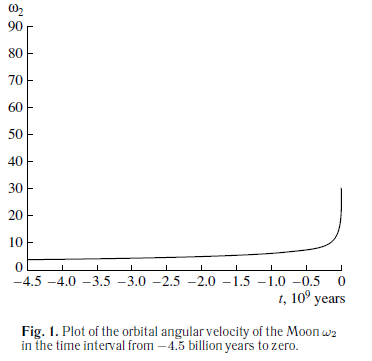
\includegraphics[width=\linewidth]{graph1.png}
  \end{subfigure}
  \begin{subfigure}[t]{0.4\linewidth}
    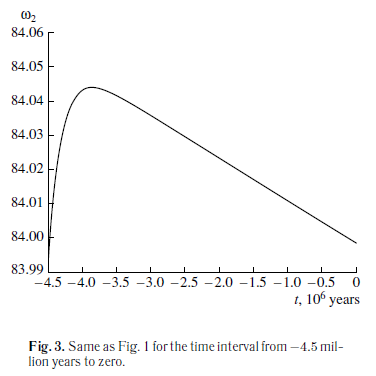
\includegraphics[width=\linewidth]{graph3.png}
  \end{subfigure}
  \begin{subfigure}[b]{0.4\linewidth}
    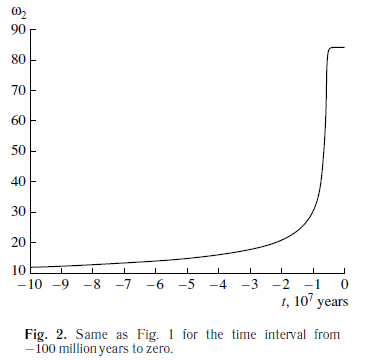
\includegraphics[width=\linewidth]{graph2.png}
  \end{subfigure}
 \begin{subfigure}[b]{0.4\linewidth}
\hbox{\hspace{+9em}
    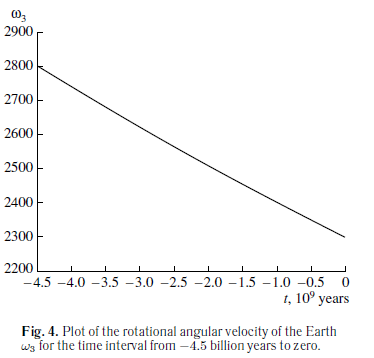
\includegraphics[width=\linewidth]{graph4.png}
}
  \end{subfigure}
\end{figure}

\begin{multicols}{2}
We can see that this differs from the value of K0 at
t = 0 given by (50) by $6 \times {10}^{-14}.$ \\
\indent As a test of the computations, the system (35) with
the input data (54) was integrated from -5 billion
years to zero. This yielded the following values at
t = 0 after this reverse computation:
$\omega_1 = 6.283185307179550,$\\
$\omega_2 = 8.399831045067062 \times 10^1,$\\
$\omega_3 = 2.294973413103788 \times 10^3,$\\
$\omega_4 = 8.399831045066902 \times 10^1.$\\
These differ from the original input data (42) in the
digits indicated in bold. The computation from zero
to -5 billion years occupied less than a minute on the
Samsung NP510R5E laptop computer used.
\indent Plots of the angular velocities for integration into
the past in the time interval from 0 to -4.5 billion
years are presented in Figs. 1-9. The horizontal
axes plot the time and the vertical axes the angular
variabiles (in the new units).
The orbital angular velocity of the Moon slowly
increases in the time interval from -4.5 billion
years to -100 million years (Fig. 1). It begins
\end{multicols}
\pagebreak

\begin{figure}[h!]
  \begin{subfigure}[t]{0.4\linewidth}
    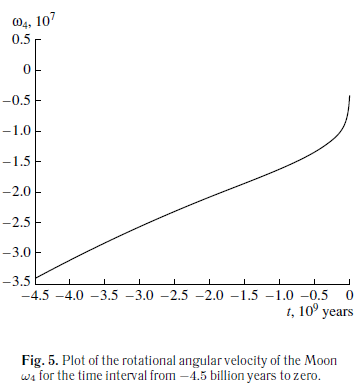
\includegraphics[width=\linewidth]{graph5.png}
  \end{subfigure}
  \begin{subfigure}[t]{0.4\linewidth}
    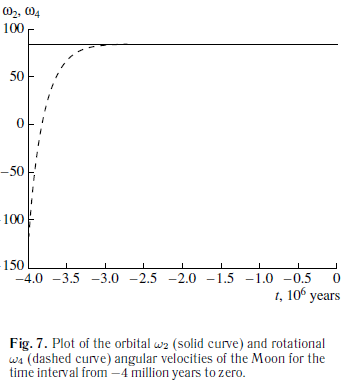
\includegraphics[width=\linewidth]{graph7.png}
  \end{subfigure}
  \begin{subfigure}[b]{0.4\linewidth}
    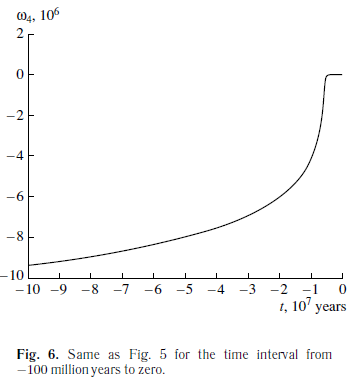
\includegraphics[width=\linewidth]{graph6.png}
  \end{subfigure}
 \begin{subfigure}[b]{0.4\linewidth}
\hbox{\hspace{+9em}
    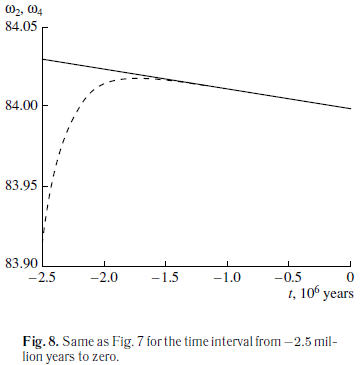
\includegraphics[width=\linewidth]{graph8.png}
}
  \end{subfigure}
\end{figure}
\begin{multicols}{2}
to grow especially rapidly from -100 million years
(Fig. 1) and from -10 million years (Fig. 2). At
t $\approx -3.852728 \times $106 years, $\omega_2$
value, $\approx $ 84.04385, then begins to decrease (Fig. 3),
as is currently observed. The rotational angular
velocity of the Earth $\omega_3$ decreases almost linearly from
$\omega_3 \approx  2.8005 \times {10}^3$ to the current value (Fig. 4). The
Moon displayed very rapid and reversed axial rotation
4.5 billion years ago. Further, over a very extended
time, the (negative) rotational angular velocity of the\\
Moon $\omega_4$ gradually increased (Figs. 5, 6). At t $\approx$
-3.817 million years, it changed sign, and the lunar
axial rotation became prograde (Fig. 7). Figures 7
and 8 show that $\omega_4$ begins to approach $\omega_2$, with $\omega_4 \approx$
83.9133 and $\omega_2 \approx 84.0295$ at t = -2.5 million years.
These two quantities have essentially become equal
at t = -1 million years:  $\omega_2 \approx  84.0108, \omega_4 \approx 84.0107.$\\
This represents a 1 : 1 lunar spin–orbital resonance,
when the lunar “day” is equal to a lunar month. This
resonance is preserved in the future, although the
\end{multicols}
\pagebreak
\begin{figure}[h!]
  \begin{subfigure}[t]{0.4\linewidth}
    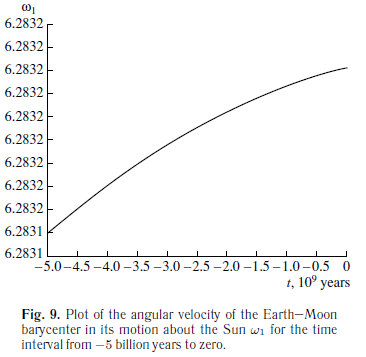
\includegraphics[width=\linewidth]{graph9.png}
  \end{subfigure}
  \begin{subfigure}[t]{0.4\linewidth}
\hbox{\hspace{+9em}
    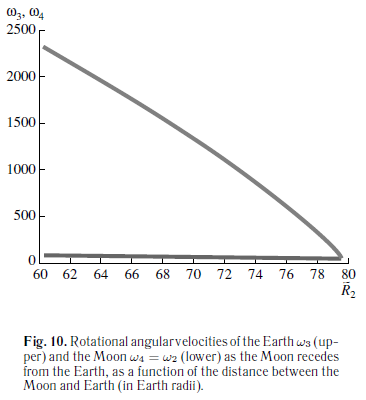
\includegraphics[width=\linewidth]{graph10.png}
}
  \end{subfigure}
\end{figure}

\begin{multicols}{2}
values of the angular variables change: $\omega_2 = \omega_4$ with
accuracy to within 2-4 digits after the decimal point;
i.e., the phenomenon of libration is observed. At
t $\approx$ -1.7330 million years, $\omega_4$ reaches its maximum
value of 84.017 and then decreases to the current
value (Fig. 8). The value $\omega_1$ changes almost linearly,
growing by$\approx 3.57 \times $10-5 from t = -5 billion years to
t = 0 (Fig. 9).\\
2. Integration into the Future Predicting the evolution
of the Earth–Moon system into the future is
even more difficult—both because we do not know the
intrinsic time frame, and because the values obtained
could be erroneous due to imperfections in our model.
Therefore, we adopted the distance between theMoon
and the Earth, taken to vary within some reasonable
limits, as an independent variable (we discuss this
question further in Section 5). \\
\indent We obtained the following system of equations of
motion from (35): \\
$\omega_1^{\prime} = c_1 \omega^{16/3}_1 [k_1(\omega_1 - \omega_3) + k_2(\omega_1 - \omega_4)]V,$ \hfill (55)
\end{multicols}
\pagebreak

\begin{figure}[h!]
  \begin{subfigure}[t]{0.4\linewidth}
    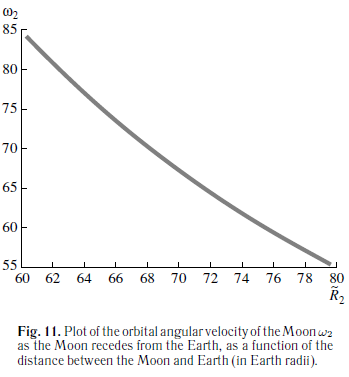
\includegraphics[width=\linewidth]{graph11.png}
  \end{subfigure}
  \begin{subfigure}[t]{0.4\linewidth}
    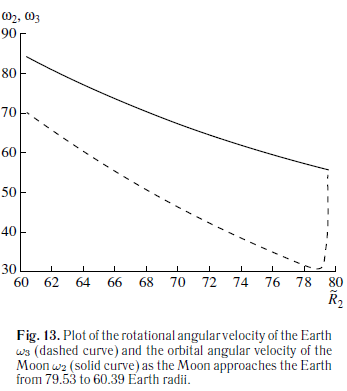
\includegraphics[width=\linewidth]{graph13.png}
  \end{subfigure}
  \begin{subfigure}[b]{0.4\linewidth}
    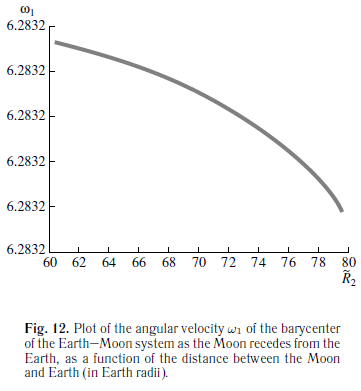
\includegraphics[width=\linewidth]{graph12.png}
  \end{subfigure}
 \begin{subfigure}[b]{0.4\linewidth}
\hbox{\hspace{+6em}
    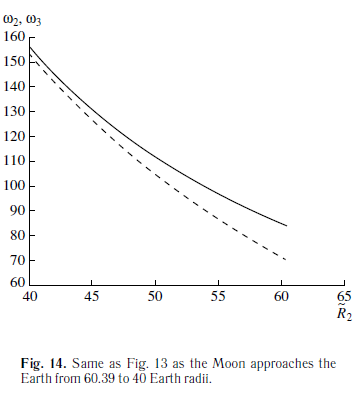
\includegraphics[width=\linewidth]{graph14.png}
}
  \end{subfigure}
\end{figure}

\begin{multicols}{2}
$\omega_4 = 55.571553739447416.$
The corresponding integral of the angular momentum, \\
$K_0 = 42.75292278673107,$
differs by $4 \times {10}^{-14}$ from the initial value (50). Here,
we can see that $\omega_3$ is now smaller than $\omega_2$\\
The following values of the angular variables were
obtained when $R_2$ = 79.530836093424753:\\
$\omega_1 = 6.283183446070644,$\\
$\omega_2 = 55.579808373540935,$\\
$\omega_3 =56.02657531218837,$\\
$\omega_4 = 55.571559310581840.$\\
The corresponding integral of the angular momentum, \\
$K_0 = 42.75292278673107,$
differs by $3 \times {10}^{14}$ from the initial value (50). The\\
\end{multicols}
\pagebreak
\begin{multicols}{2}
\begin{flushleft}
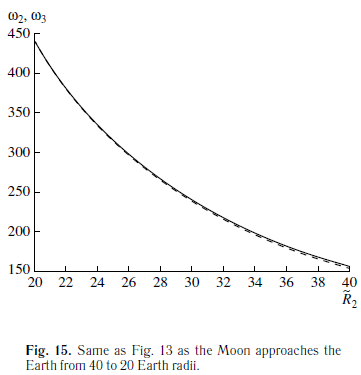
\includegraphics[width=8cm,height=5cm]{graph15.png}
\end{flushleft}
angular velocity $\omega_1$ decreased by $\approx 2 \times 10^{-6} $compared
to the initial value (42) (Fig. 12).\\
\indent We integrated the system (55) with the initial data
(58) as $R_2$ varied from 79.530790508689833 to unity;
i.e., as the Moon approached the Earth. Figures 13-
17 show plots of the variations of $\omega_2$ and $\omega_3$. In
Fig. 13, $\omega_3$ sharply decreases, reaching its minimum
value $\omega_3 \approx 30.668$ when $R_2 \approx 78.854$. At this time,
 $\omega_2 \approx 56.297.$ Further, $\omega_3$ begins to grow, remaining
smaller than $\omega_2 $.\\
\indent We observe the same picture in Fig. 14. In Fig. 15,
$\omega_2 $ and $\omega_3$ begin to approach each other, and we
have $\omega_2  \approx 440.7$ and $\omega_3 \approx $ 440.6 when $R_2$ = 20. We
observe here the resonance  $\omega_2 : \omega_3 : \omega_4 \approx 1 : 1 : 1$,
when the Earth and Moon both keep the same face
toward each other. The angular velocities $\omega_2$ and
$\omega_3$ grow, but remain equal. This continues roughly
until $R_2$ = 10, after which $\omega_2$ and $\omega_3$ begin to diverge
and increase, but with $\omega_2$ growing appreciably
faster: we have when $R_2$ = 5 $\omega_2 \approx 3525$ and $\omega_3 \approx 
2352$ (Fig. 16), and$ \omega_2 \approx 39 420$ and $\omega_3  \approx 3800$ when
$R_2$ = 1 (Fig. 17). The Moon rapidly approaches the
Earth, and collides with it when $R_2$ = 1. At that time,
$K_0$ = 42.75292278672882, which differs from the initial
value by $229 \times 10^{14}$. The angular velocity of the
barycenter of the Earth–Moon system $\omega_1$ decreases
by $\approx {10}^{-5}$ compared to the initial value (42) (Fig. 18). \\
\indent Further, to compute the distance of the Earth-
Moon barycenter from the Sun $R_1$, the distance from
the Earth to the Moon $R_2$, and the current periods of
rotation of the Earth and Moon $T_t$ (for the current rotational
angular velocity $\omega_t$), we applied the following
formulas: \\
$R_1 = \sqrt[3]{GM\omega^{-2}_1Lm},$ $R_2 = \sqrt[3]{Gm \omega^{-2}_2} L m,$ \hfill (59) \\
$T_t = 2 \pi / \omega_t Ts,$\\
where the values of the constants are given in (39),
(40). We used the resulting plots of the variations of
the angular velocities to construct the tidal evolution
of the system on cosmological time intervals.
\end{multicols}
\begin{figure}[b]
  \begin{subfigure}[t]{0.4\linewidth}
    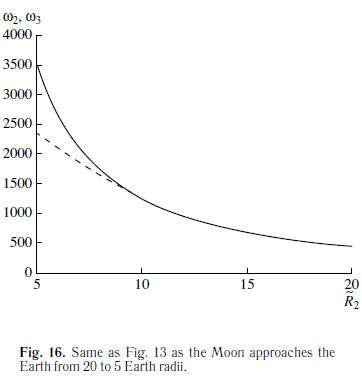
\includegraphics[width=\linewidth]{graph16.png}
  \end{subfigure}
 \begin{subfigure}[b]{0.4\linewidth}
\hbox{\hspace{+9em}
    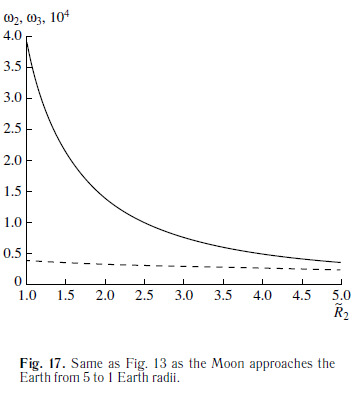
\includegraphics[width=\linewidth]{graph17.png}
}
  \end{subfigure}
\end{figure}


\pagebreak



\begin{multicols}{2}
\begin{center}
 4. TIDAL EVOLUTION\\
OF THE EARTH–MOON SYSTEM
\end{center}
\indent 4.5 billion years ago, the distance between the
Moon and the Earth was three million kilometers.
The Moon then slowly approached the Earth over a
long time interval. 500 million years ago, the Earth–
Moon distance was 1.9 million kilometers. An interval
of more rapid variation of the parameters of
motion of the Moon began about 100 million years
ago. The Moon reached its minimum distance to the
Earth about 3.9 million years ago, with this distance
differing from the distance at the current epoch by
about 150 km. The Moon then began to slowly
recede, as is observed today.\\
\indent An Earth day 4.5 billion years ago was only a few
hours shorter than the current day, 19.667 hr. Our
theory agrees with all other existing theories that the
duration of the day was shorter in the past due to
the effect of tidal friction, and the length of the day
has gradually increased over the course of the Earth’s
evolution. This is confirmed by paleontological data:
the duration of an Earth day was 21.9 hr 620 million
years ago [30].\\
\indent The Moon displayed very rapid and retrograde rotation
4.5 billion years ago. The rotational velocity of
theMoon then gradually slowed, until the direction of
the rotation was reversed 3.8 million years ago; i.e.,
the rotation direction became the same as at the current
epoch. The Moon’s rotation rate then began to
increase, and the length of the lunar “day” to shorten.
About 1.733 million years ago, the duration of the
lunar “day” reached a local minimum, differing from
the value for the current epoch by several minutes.
The lunar “day” then began to gradually increase.\\
\indent The modern history of the Moon begins roughly
one million years ago, when its orbital angular velocity
became essentially equal to its rotational velocity.
The length of the lunar “day” became equal to the
length of a lunar month; i.e., a 1 : 1 resonance was
achieved. The computations indicate that this resonance
has been preserved over the entire evolution of
the Moon. \\
\indent Laser observations indicate that the Moon is currently
receding from the Earth [28]. In the future,
the duration of the Earth day and the lunar month
(lunar day) will smoothly grow, but the Earth day
will remain shorter than the month. At a distance of
about 506 692 km—the maxinum distance between
the Moon and the Earth —they will become comparable
and equal to 41.29 d. Further, theMoon will begin
to gradually approach the Earth, and the lunar day
will begin to decrease while the Earth day increases.
At an Earth–Moon distance of 502 380 km, the rotation
period of the Earth will reach its maximum value
of 74.8 d and the rotational period of the Moon will
be 40.8 d, after which the Earth day will begin to
\begin{flushright}
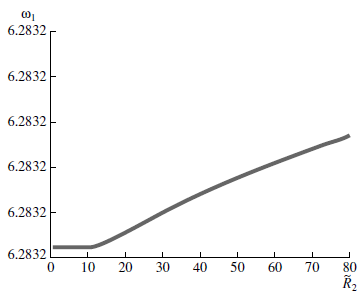
\includegraphics[width=8cm,height=5cm]{graph18.png}
\end{flushright}
decrease, remaining longer than a lunar month. The
motion of the Moon back toward the Earth can be
explained by tidal theory [1, 31]: since the month is
shorter than the rotational period of the Earth, the
effect of tidal friction begins to draw the Moon back
toward the Earth. Our results are also supported by
other theories [2, 3]. Goldreich [3] has written that,
since the lunar tidal torque exceeds the solar tidal
torque at a maximum distance of 75 Earth radii, and
since the Moon’s orbital moment of inertia exceeds
the Earth’s, the rotation of the Earth will begin to
be accelerated while theMoon approaches the Earth,
with the Earth day always remaining slightly longer
than the month. \\ 
\indent
The approach of the Moon toward the Earth and
the increase in the Earth’s rotation rate will mean
that the Earth day and the lunar month approach
each other and decrease sharply. They both become
equal to about 5.21 d at a distance of about 20 Earth
radii. This testifies to synchronization of the motions;
i.e., $\omega_2 \approx \omega_3 \approx \omega_4$, so that the Earth and the Moon
keep their same faces toward each other. However,
although the angular velocities are equal, they are
not constant, and increase. This synchronization is
unstable, and becomes disrupted at distances of less
than 10 Earth radii. As before, $\omega_2$ is equal to $\omega_4$ . The
Moon approaches the Earth, its orbital velocity appreciably
exceeds the rotational velocity of the Earth;
ultimately, the Moon passes inside the Roche limit at
a distance of less than three Earth radii, is disrupted,
and collides with the Earth. \\
\indent During this expansive evolution, the radial distance
of the barycenter of the Earth-Moon slowly\\
increases, increasing by $\approx $ 224 km by the end of the
evolution, compared to its value at t = 0.
\end{multicols}
\pagebreak
\begin{multicols}{2}
\begin{center}
 5. DISCUSSION AND CONCLUSION
\end{center} 
~\indent The evolutionary picture described above is hypothetical,
and we do not know exactly to what points in
the past and the future it is correct. We have considered
the evolution only of the four angular velocities
characterizing the distance between the barycenter of
the Earth–Moon system and the Sun and between
theMoon and the Earth, and the axial rotations of the
Earth and theMoon. Let us consider the basis for the
applicability of our model.\\
\indent Cosmological time intervals of several billion years
are rather long for studies of the evolution of the
Earth–Moon system. Therefore, it is unlikely that
all the variables changed in a continuous fashion
during the evolution of this system. It is known
from paleontological data that there have been several
epochs of mass extinction on the Earth in the past.
This suggests that the tilt of the Earth’s axis could
experience jumps, possibly including a reversal of the
poles. This could lead to changes in the direction and
rate of the Earth’s rotation. Thismeans that, however
accurate a model may be, we cannot be confident
of the correctness of our results further than 12 000
years in the past (the epoch of the latest catastrophe,
the worldwide flood). If we consider a time interval of
4.5 billion years, the mean position of the Earth’s axis
has been perpendicular to its orbital plane.\\
\indent Another theoretical basis is the fact that, in the
motion of the center ofmass of a viscoelastic planet in
a central force field, its rotational axis will tend to become
oriented perpendicular to its orbital plane [20].
In relation to this reasoning, the Moon’s rotation axis
is also assumed to be perpendicular to the plane of its
orbit. Since the Earth’s equator could unpredictably
change its position, the angle between the Moon’s
orbital plane and the Earth’s equator could also vary
unpredictably. The mean value of this angle is taken
to be zero. \\
\indent  It is known that the limiting motion of the center
of mass of a viscoelastic planet in a central force
field is circular [19]. Therefore, in our model, the
barycenter of the Earth-Moon system moves around
the Sun in a quasi-circular orbit over cosmological
time intervals, and the Moon likewise moves about
the Earth in a quasi-circular orbit; i.e., along winding
or unwinding spirals. \\
\indent On the one hand, our celestial mechanical model
is simple in the sense that it has relatively few parameters,
due to the difficulty of the problem that
we wish to solve. On the other hand, it can be
considered complex. A Kelvin–Voigt model has been
adopted for viscous forces. The bodies are spheres in
their unperturbed motion, and compressed along their
rotational axes in their perturbed motion, with their
surfaces taking on complex shapes due to the action
of viscous, dissipative forces. Naturally, the shapes of
the bodies are continually changing as the parameters
of their motion change. The influence of the oceans
on the surface of the Earth has not been taken into
account at all. The study of Krasinsky [32] casts
doubt on the hypothesis that the main contribution
to the tidal dissipation of the Earth is made by the
oceans. \\
\indent Let us now consider the time scales for the evolution
of the Earth and Moon. The coefficients $k_1$
and $k_2$ from (36), which appear in the equations of
motion, are integrated coefficients characterizing the
viscoelastic properties of the Earth and Moon. We
calculated their values at the current epoch, based
on available astronomical data. However, their values
will change with time in reality, and in ways that are
not known. This could not only disrupt the chronology,
but also provide the main reason for discrepancies
between the model and physical reality. In other
theories, lack of knowledge of the true variations in
the dissipative function Q associated with the timedependent
delay angle, the relative angular velocity
of the rotations of celestial bodies, and other factors
have made it necessary to assume that the delay angle
is constant in a first approximation. As was shown
in [2], the epoch of the maximally close approach of
theMoon to the Earth occurred 1.79 billion years ago,
when this distance was 2.72 Earth radii. This means
that theMoon was inside the Roche lobe, and subject
to disruption. Such a short “lifetime” for the Moon
is in contradiction with available paleontological data
[33] and the results of lunar expeditions. It is noted
in the later work of Kaula [34] concerning dynamical
aspects of the origin of the Moon that, if the rate of
recession of the Moon from the Earth has been constant
throughout its history, the Moon should have
been dangerously close to the Earth only 1.75 billion
years ago. Krasinsky [6] suggests that Q must have
grown with time in the past. \\
\indent Integrating into the past, we restricted our analysis
based on available data on the ages of the Earth
and Moon, 4.5 billion years. In this case, we do not
encounter the problem of the small time scale for the
evolution of the lunar orbit, which the theories indicated
above cannot resolve. The minimum distance
between the Moon and Earth is only about 150 km
smaller than their current separation. It follows from
the evolution of our system that the origin of the Moon
may not be related to the Earth, and it is quite likely
that it formed in another region of circum-solar space. \\
\indent For this reason, the hypothesis of Darwin [35]
that the Moon separated off from the Earth and the
giant-impact hypothesis [36] are not supported by 
\end{multicols}
\pagebreak
\begin{multicols}{2}
our results. A number of other theories in which the
age of the Moon is substantially less than 4.5 billion
years are likewise not supported. We have studied
the evolution of the rotational motion of the Moon
for the first time here. Our results suggest that the
axial rotation of the Moon was initially opposite to
its current direction. The current character of the
Moon’s motion developed several million years ago,
when its rotation became prograde, it approached the
Earth to a minimum distance, and then began to
recede, entering into a 1 : 1 resonance at subsequent
times.\\
\indent Integrating the equations ofmotion into the future,
we encountered an unrealistic time scale (due to the
above comments concerning the coefficients k1 and
$k_2$), although the qualitative run of events is supported
by theory [2, 3]. Based on this, we can express
some events in terms of others. What should we be
guided by in this case? Our theory yields a maximum
distance between theMoon and Earth of 79.53,
the theory of MacDonald [2] 72.5, and the theory of
Goldreich [3] 75 Earth radii. These values are similar
and realistic. Therefore, we expressed the remaining
three variables in terms of the distance between the
Moon and Earth, and represented the evolutionary
picture into the future as a function of the radius of the
lunar orbit and the recession from or approach toward
the Earth. After reaching its maximum separation of
506 662 km, the Moon begins to approach the Earth.
In the penultimate stage of the evolution, an unstable
1 : 1 : 1 synchronous resonance with the rotation
of the Earth is added to the spin–orbit resonance of
the Moon; this is then subsequently disrupted due
to the sharp increase in the orbital angular velocity
of the Moon. In the final stage, there is a close
approach of the Moon toward the Earth ending with
a collision. The same tidal-evolution mechanism is
moving Phobos closer to Mars. Its orbital angular
velocity, which is synchronized with its rotation, exceeds
the rotational angular velocity ofMars by nearly
a factor of three. This is what is predicted by our
theory in the final stage of approach of the Moon
and the Earth. According to the computations of
Efroimsky and Lainey [8], Phobos will impact Mars
in 40–43 million years. Deimos is currently receding
from Mars, and it would be interesting to try to predict
its evolution into the future. \\
\indent In contrast to all the theories referred to above, we
have considered the evolution not only of the orbital
motion of the Moon, but also the evolution of the
Earth–Moon barycenter. Tidal evolution led to an
increase in the barycenter distance by 224 km. Based
on an analysis of more than 635 000 observations
of planets and spacecraft, primarily radio-technical
data (1961–2010), Pit’eva and Pie’ev [37] derived
the rate of variation of the heliocentric gravitational
constant. Their results indicate that the barycenter of
the Earth–Moon system is receding from the Sun at
an average rate of 1 cm/year. Tidal evolution clearly
makes a significant contribution to this process. \\
\indent Thus, we conclude that our celestial-mechanical
model with relatively few parameters is able to scientifically
describe the tidal evolution of the Earth–
Moon system over cosmological time intervals in a
first approximation. The model does not include
many physical processes, but nevertheless can provide
qualitatively important results without invoking
other complex theories. The most debatable issue
is the origin of the Moon, which currently remains
unresolved. Themain conclusions given by ourmodel
are supported by astronomical observations, paleontological
data, and studies based on other theories.
We have also presented the possible evolution of the
rotational motion of theMoon for the first time.\\

\end{multicols}
\thispagestyle{fancy}
\fancyhead[L]{TIDAL EVOLUTION OF THE EARTH–MOON SYSTEM}

\end{document}